
%Superscripts and subscripts that are words or abbreviations, as in
%\( \pi_{\mathrm{low}} \), should be typed as roman letters; this is
%done as \verb|\( \pi_{\mathrm{low}} \)| instead of \( \pi_{low} \)
%done by \verb|\( \pi_{low} \)|.

%User-defined macros should be placed in the preamble of the chapter,
%and not at any other place in the document. Definitions made using
%the commands \verb|\newcommand,| \verb|\renewcommand,|
%\verb|\newenvironment| or \verb|\renewenvironment| should be used


\chapter[Cyclotron]{Cyclotron}\label{chapCyclotron}


\section{Introduction \label{secCycloIntro}}

In a Universe of, at that time, electrostatic accelerating devices, which included the recent Wideroe's linac~\cite{TBRef'd},  
the cyclotron marks the coming age of circular accelerators. The concept is due to E.~O.~Lawrence and dates form 1932, 
it was  that of a  magnetic field, constant in time, in a region between to magnetic poles 
including a double-Dee system that creates a pair of  gaps in which a 
constant-frequency accelerating RF voltage is applied (Fig.~\ref{figLBLCycloSketch}).  
In that sense it was understood by its inventor as a  ``folded linac'', 
a circular accelerator structure~\cite{TBRef'd},  
allowing  repetitive  passes through a single accelerating device. 


\begin{figure}[ht]
\centering
\sidebyside
{
    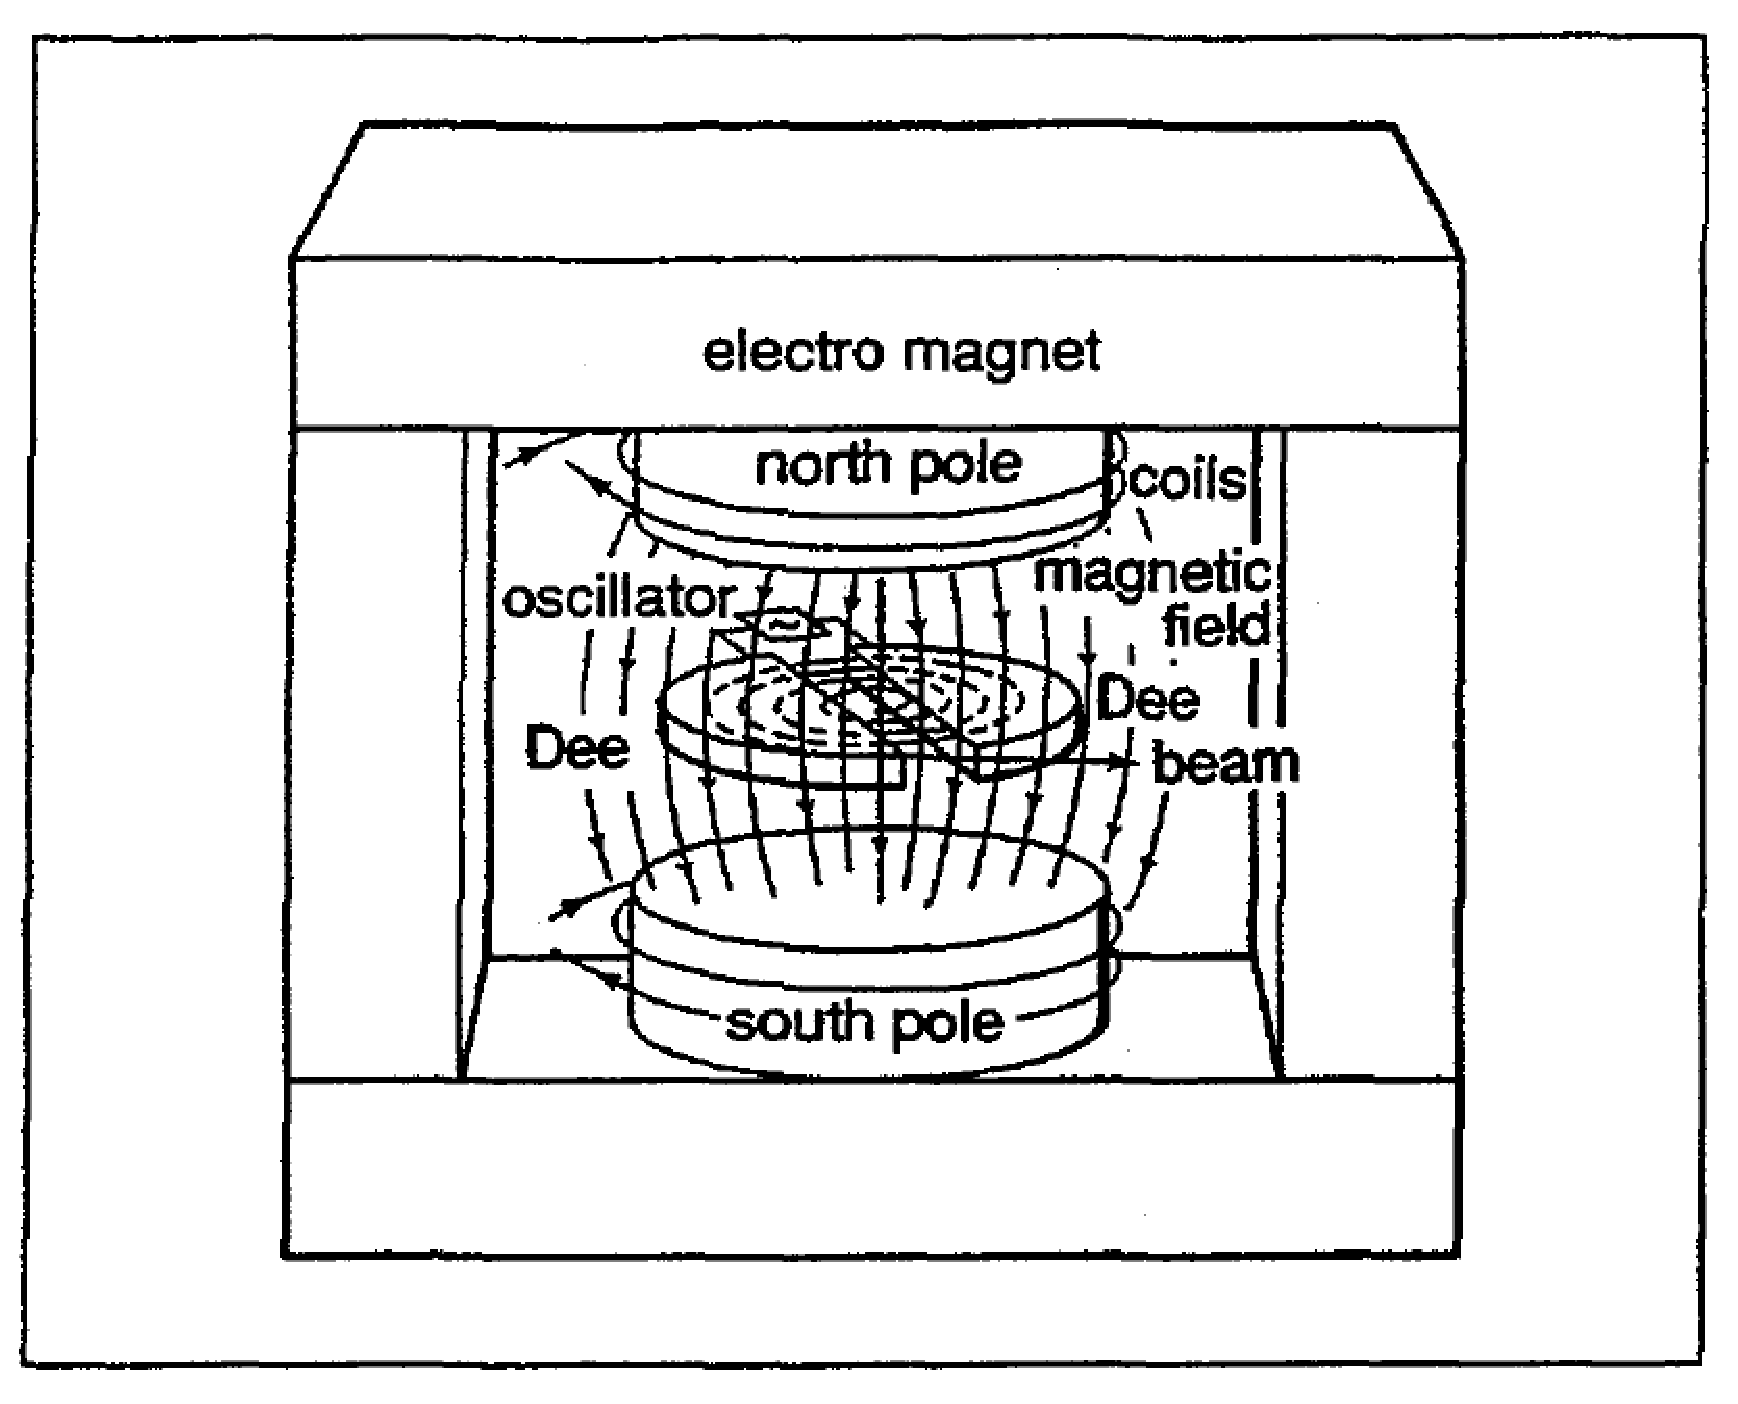
\includegraphics[width=0.45\linewidth]{./figs_cyclo/LBLCycloSketch.eps}
    \caption{A  resonant acceleration device: the cyclotron~[1].} %\cite{CASCycloSketch1994}    
\label{figLBLCycloSketch}
}{
    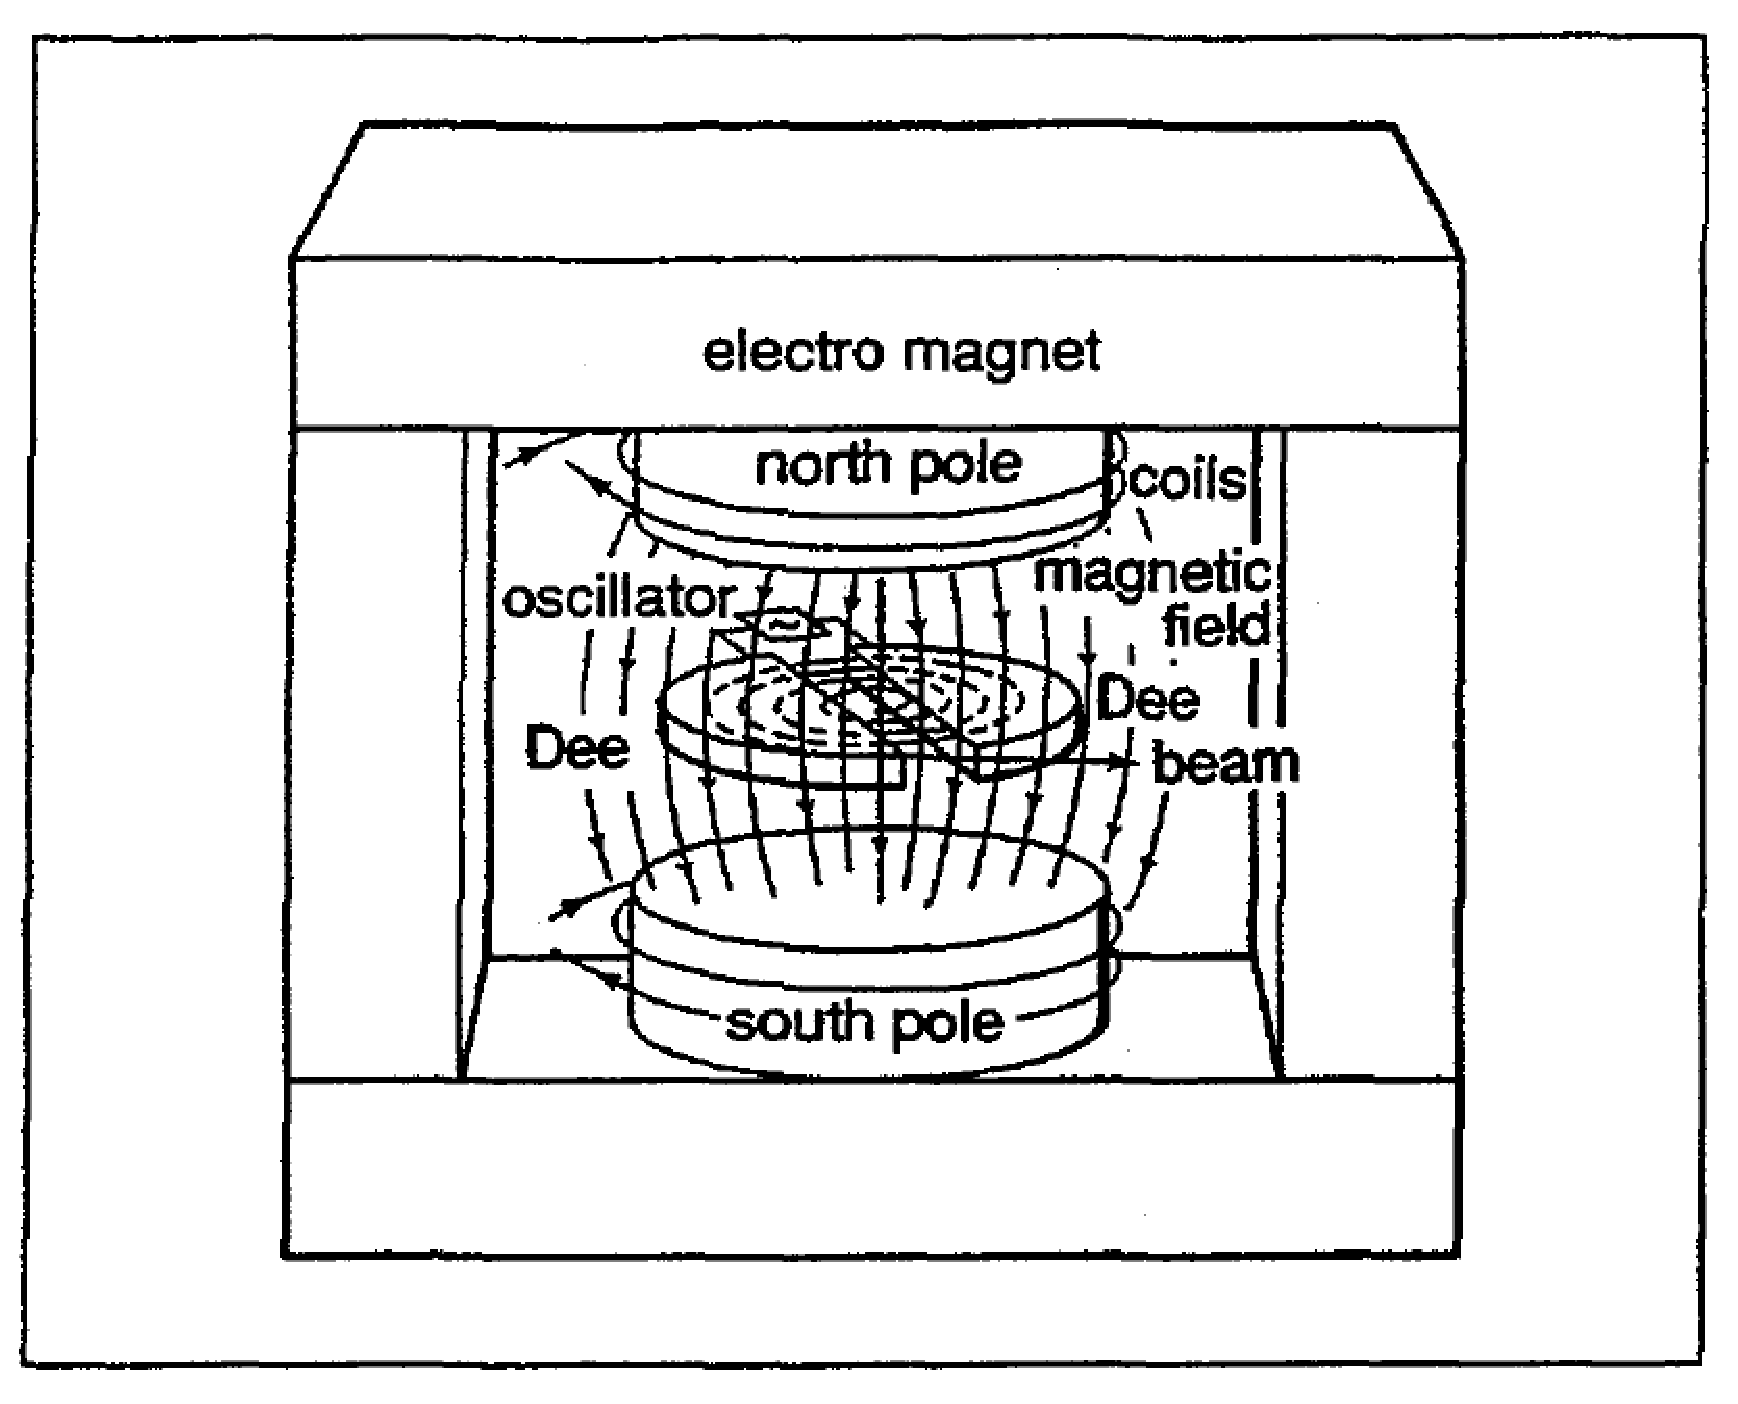
\includegraphics[width=0.45\linewidth]{./figs_cyclo/LBLCycloSketch.eps}
    \caption{     The world highest beam power cyclotron, at PSI.}
\label{figPSICyclo}
}
\end{figure}

\subsubsection*{Principle}

In that region of uniform field $B$ a  particle with rest mass $m_0$, 
relativistic mass $m=\gamma m_0$, charge $q$, momentum $p=mv$, undergoes a circular motion
characterized by its radius $R$, with a revolution period $T_{\rm rev}$ which depends on the field 
and on the particle charge and mass, but \emph{not} on $R$ neither on the particle velocity. 
Thus repeated acceleration can be provided by a system (the double-gap formed by the double dee in Fig.~\ref{figLBLCycloSketch}) 
with fixed frequency $f_{\rm RF}$ in resonance, at some harmonic integer $h$, 
 with the orbital frequency $f_{\rm rev}=T^{-1}_{\rm rev}$ of the particle. These three quantities satisfy, respectively 
\begin{equation}
\label{EqRCyclo}
 R = p / qB, \hspace{.1\linewidth} 2\pi f_{\rm rev} = v/R = q B / m, \hspace{.1\linewidth} f_{\rm RF} = h f_{\rm rev}
\end{equation}

These expressions hold in both cases of  \emph{classical} cyclotron, which  operates in 
 sub-relativistic regime ($\gamma m_0\sim m_0$), 
and  \emph{isochronous} cyclotron which operates in  relativistic regime ($\gamma $ distant from 1).  


\paragraph {\sl Recommended readings,} in order to prepare this exercise series:

Cyclotron: bibliography documents listed in page~\pageref{SecBiblioCyclotron}.

Zgoubi Users' Guide~: (i)~applied mathematics methods i sections: 1.2, 1.3.3, 1.4,  
complete/strengthen with classical Applied Mathematics textbooks. (ii)~DIPOLES procedure and ancillaries.



\section{Classical cyclotron \label{secCycloClass}}

Fixed-frequency acceleration requires  matching between the RF and cyclotron frequencies. 
However the relativstic increase of the mass causes the 
 the revolution period to change with energy, $\Delta T_{\rm rev}/T_{\rm rev} = \gamma-1 $.  
The mis-match between the accelerating and cyclotron frequencies 
sets a limit to the highest velocity, $\beat=v/c\approx 0.22$,  $\rm \Delta T_{\rm rev}/T_{\rm rev} \approx 2-3$\%.  
This means a maximum $E-mc^2 \approx$25~MeV kinetic energy for protons, 50~MeV for D and $\alpha$ particles. 
%That is enough energy to transmute all nuclei and, as a matter of fact, the classical cyclotron allowed discovering 
%numerous nuclear reactions and isotopes. 

The classical cyclotron  is comprised of, (i)~a cyclindrical dipole magnet which provides a uniform 
 magnetic field between its two poles, (ii)~two semi-cylindrical dees inserted 
in the empty region between the  poles, connected to an alternating current (AC) source. 
Inside the dees, ions only experience the magnetic field, in the two gaps between the dess, ions 
experience an accelerating force, at each passage across a gap due to the alternating polarity of the AC source.



\subsection{Closed orbit, time of flight \label{secCycloClassOrb}}

A cyclotron accelerator is a typical case 
where just putting together drifts and dipoles in a matrix transport works at best 
at a particular energy and for paraxial motion, yet won't permit designing an accelerator. 

The common solution is to use a field map. However, mathematical models for the field 
are also a good approach in a preliminary design phase due to the flexibility it brings 
in parameters as orbit excursion, isochronism, focusing, etc.

These two techniques are employed  in the exercises, to develop on the properties of particle motion 
in cyclotrons. 

\smallskip
\noindent {\small $\bullet$} Exercise~\ref{secCycloClassOrb}-1 

\noindent ~\ref{secCycloClassOrb}-1.a - 
Construct a 60-degree sector mid-plane 2-dimensional field map, with constant vertical field 
B=0.5~T, covering R=10 to 70~cm. Take for that a uniform mesh in cylindrical coordinates proper for use 
with \texttt{TOSCA} option ``IZ=1, MOD=22, MOD2=1''. 
Using \texttt{TOSCA} keyword, track three protons with energy respectively 0.2, 1 and 5~MeV,
launched a zero angle into the field map. 
Check that trajectories are arc of circles, at expected radii. 

\noindent ~\ref{secCycloClassOrb}-1.b - 
 Plot, as a function of energy, the 
  radius $R$ and  time of flight $T_{\rm rev}$ on that orbit, 
 from both ray-tracing and kinematics theory, on a same graphic, 
showing   the slow, relativistic TOF increase with momentum. 

\noindent ~\ref{secCycloClassOrb}-1.c - 
Check the evolution of orbit radius and TOF  with field map mesh density and with 
integration step size.



\smallskip
\noindent {\small $\bullet$} Exercise~\ref{secCycloClassOrb}-2 
 \verb|CYCLOTRON| or \verb|DIPOLE| are two procedures amongst others, that provide an analytical 
 magnetic field model ${B_y(r,\theta)|_{y=0}}$ in the median plane of a dipole magnet. 
Use it to simulate a uniform field ring and re-derive the results above. 
From the two series of results, comment on various pros and cons of the two methods, analytical field models and 
fieldmaps.

\medskip

\noindent \textsl{Periodic motion -} 
Horizontal motion in a  cyclotron defined using six such 60$^o$ sectors has no priviledged reference orbit, 
for a given momentum, the initial radius and velocity vector define a closed, circular orbit.  
A particle launched with a vertical velocity component on the other hand, drifts linearly with time, as there is no 
vertical restoring strength component. The next Section will investigate the missing field property, 
for  periodic motion stability. 


\smallskip
\noindent {\small $\bullet$} Exercise~\ref{secCycloClassOrb}-3 
Observe the first statement above by tracking  particles with different initial velocity vector in a 6-sector ring. 
Plot their trajectories. 
Observe the second statement by plotting the vertical coordinate  of a particle launched with a 
vertical initial velocity component. 



\subsection{Focusing  \label{secCycloFocus}}

Let $B_r$, $B_y$  be the radial and axial components of the magnetic field, respectively, 
$x=r-R$ a small radial displacement with respect to the reference circular orbit at R,  
$\omega_{\rm rev} = 2\pi f_{\rm rev} $ the angular frequency of the circular motion. 
The radial and axial  strengths experienced by a particle moving in the vicinity of that reference orbit 
write, to the first order in the radial, $x$,  and axial, $y$, coordinates 
\begin{eqnarray}
\label{EqCycloFoc}
\rm
F_x = & m \ddot x=&  -qvB_y + m\frac{v^2}{r} \approx -q v (B_y|_{x=0} + \frac{\partial B_y}{\partial r}x)  + m\frac{v^2}{R}(1-\frac{x}{R}),   \nonumber \\ 
\rm 
F_y= & m\ddot y = &  qvB_r \approx q v \frac{\partial B_r}{\partial y} y = q v \frac{\partial B_y}{\partial r} y
\end{eqnarray}
These relations yield the differential equations for the raidal and axial motions, respectively, 
\begin{eqnarray}
\label{EqCycloDiffEq}
\rm
  \ddot x + \omega_r^2 x=0 &  \ \ \ \ \ \ \ \rm and \ \ \ \ \
  \ddot{y} - \omega_y^2 y= 0  
\end{eqnarray}
wherein 
$\omega_r^2 = \omega_{\rm rev}^2(1+\frac{R}{B}\frac{\partial B_y}{\partial r})$,  
$ \omega_y^2 = \omega_{\rm rev}^2 \frac{R}{B} \frac{\partial B_y}{\partial r}$. 
Focusing by a restoring force appears owing to the use of a magnetic field with radial 
index 
\begin{equation}
\label{EqCycloRadialIndex}
k = \frac{R}{B}\frac{\partial B_y}{\partial r}|_{x=0,y=0} 
\end{equation}
The two quantities 
\begin{equation}
  \nu_r = \omega_r/\omega_{\rm rev} = \sqrt{1+k},   ~ ~ ~ ~ 
 \nu_y=\omega_y /\omega_{\rm rev}  = \sqrt{-k} 
\end{equation}
are known  as, respectively, the radial and axial ``wave number'' of 
the oscillatory motion around the reference circular orbit of radius R.

\smallskip
\noindent {\small $\bullet$} Exercise~\ref{secCycloFocus}-1
Plot two particle trajectories that demonstrate the value of the radial wave number in a uniform 
field. Conclude on orbit and horizontal motion  stability. 
Derive the horizontal and vertical  transport matrices from ray-tracing, conclude on the stability of the 
 motion in a uniform field.


\paragraph{\sl Periodic stability  \label{secCycloPerStab} - }
Vertical motion stability requires $k$ to be negative~:  $B_y$ (respectively, the magnet gap) 
has to  slowly  decrease (increase) with radius, so resulting restoring force toward the median plane. 
Stability of both radial and axial motions requires $-1 < k <0$, a conditon known as ``weak focusing''.
 Note that  at low energy  the electric field in the 
region of the accelerating gap also contributes to the focusing, an aspect which will be omitted here. 


\smallskip
\noindent {\small $\bullet$} Exercise~\ref{secCycloFocus}-2
Back to the field map of exercise~\ref{secCycloClassOrb}-1, or to the analytical model 
of exercise~\ref{secCycloClassOrb}-2: introduce a field index $-1<k<0$ in this sector field. 
Plot the radial and vertical paraxial motions of a 3~MeV ion over a few turns. 
Compute its radial and axial motion wave numbers, $\nu_r$ and $\nu_y$, 
using two different methods, namely, 1-turn mapping and  Fourier analysis of few tens of turns. 


\smallskip
\noindent {\small $\bullet$} Exercise~\ref{secCycloFocus}-3
Using either the field map or the analytical model devised in the  exercise~\ref{secCycloFocus}-2, 
 plot the energy dependence of the reference orbit radius, $R(E)$. 
Show that $\nu_r^2 + \nu_y^2=1$, at all radii.


\paragraph{\sl Phase space motion  \label{secCycloPhasSpac} }
 is the solution of the equations of motions (Eq.~\ref{EqCycloDiffEq}). 
It satisfies (with z standing for x or y)
\begin{equation}
\label{EqCycloInvariant}
\rm
\gamma_z z^2 + 2 \alpha_z z z' + \beta_z z'^2 = \epsilon/\pi
\end{equation}
{\sl i.e.}, phase space coordinates lie on an ellipse with surface $\rm \epsilon$.  
$\rm \epsilon/\pi$ is known as the ``Courant invariant''~\cite{Courant}. 


\smallskip
\noindent {\small $\bullet$} Exercise~\ref{secCycloFocus}-5
On a common graphic, plot the horizontal phase space portrait of 0.2, 1, 3 and 50~MeV particles
taken on $\epsilon_x = \epsilon_y = 1\ \pi\mu$m invariant in each case.
Plot the vertical phase space motion for these very energies. 
Plot the components of the field vector experienced by a particle as a function of 
azimutahl angle, over a few turns.



\paragraph{\sl Beam envelopes  \label{secCycloEnvlps} }
satisfy 

\smallskip
\noindent {\small $\bullet$} Exercise~\ref{secCycloFocus}-4
From multi-turn tracking, generate the envelope of a 3~MeV beam around the ring cyclotron.  


\paragraph{\sl Isochronism  \label{secCycloIsochro} - }  
The  condition  for vertical focusing, $-1 < k <0$ 
%  \hspace{2ex} \raisebox{-20mm}[0mm][0mm]{ \includegraphics[width=6cm]{rfCyclo.eps}} \\
spoils the isochronism: the guiding field $B$ and thus $\omega_{\rm rev} = qB/m$ decrease with R (with increasing momentum). 
 As a consequence, the arrival time of a particle at the RF gap (by 
extension the ``RF phase'') is not constant  (ABCDE path)


\smallskip
\noindent {\small $\bullet$} Exercise~\ref{secCycloFocus}-4
Plot the time of flight for  the sector magnet with field index. 





\section{Relativistic cyclotron \label{secCycloRel}}

The bad news with relativistic energies, is, 
the cyclotron resonance $\omega_0 = qB/\gamma m_0$, with $R = \beta c / \omega_0$  yields  
\begin{equation}
\label{EqCycloReson}
  k = \frac{R}{B}\frac{\partial B}{\partial R} = \frac{\beta}{\gamma} 
  \frac{\partial \gamma}{\partial \beta} = \beta^2 \gamma^2 
\end{equation}
$k$ is positive and increases with energy, 
 the weak focussing condition $-1<k<0$ is not satisfied. 

The time of flight on the equilibrium orbit, momentum $p = qB\rho$ and circumference $\mathcal{C}$, is 
$T =  \mathcal{C}/ \beta c = 2\pi \gamma m_0 / qB$. 
    Isochronism requires $p$-invariant time of flight, $dT/dp=0$. Differentiating the previous expression,
this requirement yields 
\begin{equation}
\label{EqCycloBgamma}
B(R) = \frac{B_0}{\gamma_0} \gamma(R)
\end{equation}
with $B_0$ and $\gamma_0$  some refence conditions and time of flight $T_0 = (2\pi m_0/q)(\gamma_0/B_0)$.

In other words, isochronism requires $ B(r) \propto \gamma$, which yields vertical defocusing. 
That was the end of the story in the late 1930s. 
Hans Bethe (1937)~: 
``... it seems useless to build cyclotrons of larger proportions than the  
existing ones... an accelerating chamber of 37 cm radius will  suffice to 
produce deuterons of 11 MeV energy which is the highest possible...''. 
Frank Cole~: ``If you went to graduate school in the 1940s, this inequality ($−1 <
k < 0$) was the end of the discussion of accelerator theory.''

  Until...

\subsection{Thomas focusing}

In 1938, L.H.~Thomas, ``The Paths of Ions in the Cyclotron'', 
introduces  edge focusing, which is based on separate bend sectors. 
% \hfill  \raisebox{-20mm}[0mm][0mm]{ \includegraphics[width=5cm]{cyclo_Baartman_p6.eps}}
In  1954, Kerst introduces the spiral sector dipole of which the spiral edge increases vertical focusing further, namely
\begin{equation}
\label{EqCycloThomasFoc}
\nu_z = \sqrt{-k + F^2(1 + 2 \tan^2 \xi)}, ~ ~ {\rm F=Flutter} = \frac{<B^2> - <B>^2}{<B>^2}
\end{equation}
% \hspace{1ex}  \raisebox{-25mm}[0mm][0mm]{ \includegraphics[width=4.8cm]{cyclo_Baartman_p7.eps}}
Edge focussing removes the weak focussing isochronism conditions: it allows  $B(R)\propto\gamma(R)$ 
 (Eq.~\ref{EqCycloBgamma}), while  ensuring vertical focusing.  

  Modern cyclotrons still  rely on these principles,
%\includegraphics[width=10cm]{cycloSpiralOuvert.eps}
%\hspace{0mm}\raisebox{-50mm}[0mm][0mm]{\includegraphics[width=18cm]{cycloMedic-proton_solution_1.eps}}
their limit in energy resides in achievable field strength and magnet size. 



\section{Resonant acceleration \label{secCycloClassAccel}}

An oscillating radio-frequency (RF) electric field 
is applied in the gap between the two dees (the electrodes, 
 ``Oscillator'' region in Fi.g~.ref{figLBLCycloSketch})
so creating a potential difference 
\begin{equation}
\label{EqRFCyclo}
 V(t) = qV sin(2\pi f_{\rm RF}t)
\end{equation}
An  ion reaching the gap at time $t$  experiences an accelerating force $\vec = -q \vec{grad}V(t)$ which changes 
its  kinetic energy by the amount $\Delta W = q V \sin(2\pi f_{\rm RF}t + \phi)$. 
With the  RF frequency satisfying $f_{\rm RF} = h f_{\rm rev}$,   the ions undergo acceleration at each passage across each gap. 


.....

     Bunching~: particle beam injected into the cyclotron necessarily gets bunched, at the 
frequency (or a sub-harmonic) of the RF, 
the time interval between two bunches is an RF period (or a multiple).




\subsection{Classical cyclotron, $0<n<1$}


Isochronous cyclotron, $0<n<1$ cannot be satisfied as $B\propto \gamma$. Introduce Thomas focusing, using sector magnets,
no longer slow r-decrease, weak focusing uniform field.



The RF gap provides a voltage  
\begin{equation}
\label{EqRFVolt}
V_{\rm RF}(t) =\hat V \cos ........... 
\end{equation}
Particles are accelerated as long as they reach the gap when the RF phase is in the 
interval $[-90,+90]$~degree. 
The closer the RF phase to $\phi=90$~deg, the smaller the number of turns 
(the time interval) necessary to reach the top energy. 
A deviation of the field B from the isochronous value $2\pi m f_{\rm rev}/q$
will result in a  shift in the arrival phase of the particle at the RF gap amounting to 
\begin{equation}
\label{EqPFPhaseCyclo}
\Delta (\sin \phi) = 2\pi h n \Delta B/B
\end{equation}

 ******* prendre de valeurs R, B, etc. realistes, e.g. in ../biblio/22047216.pdf, 23001796.pdf*******

\smallskip
\noindent {\small $\bullet$} Exercise~\ref{secCycloClassAccel}-1 

Using \texttt{CAVITE}, install a double RF gap as in Fig.~\ref{figLBLCycloSketch}, 
with a peak gap voltage $\hat V = 10$~kV, in a 6-sector ring based on the earlier material (ex.~~\ref{secCycloClassOrb}-1,~2). 
Set the RF gap parameters such that acceleration is independent of RF phase.
Track a proton from 1 to 5~MeV. Plot the path length and time of flight as a function of energy, 
compare with the results from ex.~~\ref{secCycloClassOrb}-1,~2.


\smallskip
\noindent {\small $\bullet$} Exercise~\ref{secCycloClassAccel}-2 

\noindent \ref{secCycloClassAccel}-2.a - 
Set \texttt{CAVITE} parameters to obtain the phase dependence, 
and assume an RF frequency $f_{\rm RF}$ which is the harmonic $h=$ of the revolution frequency.
Track a proton from 1 to 5~MeV. 
Get the path length, time of flight, RF phase as a function of energy,
compare with the results of exercise~\ref{secCycloClassAccel}-1.

\noindent \ref{secCycloClassAccel}-2.b - 
Introduce a magnetic field defect $\Delta B/B= 10^{-4}$, uniform over the ring. 
In a $V(\phi)$ diagram, represent  the arrival phase  of the particle at the RF gap
by plotting it along the V(t) curve. 
Compare the evolution time of flight, RF phase, number of turns to the top energy,
 with the results of 2.a above.
 Plot the final phase $\phi_{\rm final}$ as a function of $\Delta B/B$. 
 Find the tolerable deviation from the isochronous field, 
$\Delta B/B$,  if particles are required to be dispersed in momentum by les 
than $dp/p=10^{-3}$ at the end of the acceleration cycle.




\subsection{Relativistic cyclotron}




\section{Bibliography \label{SecBiblioCyclotron}}

Stambach CAS

R Baartman Cyclotrons: Classic to FFAG

 Courant article
